\documentclass[pdftex,12pt,fullpage,oneside]{amsart}
\usepackage{array,amsmath,psfrag,amssymb,subfigure,tabularx}
\usepackage{hyperref,multicol}
\usepackage{booktabs}
%\usepackage{vmargin,boxedminipage}
\usepackage[usenames]{color}
\usepackage{datetime}
\usepackage{dcolumn}
\usepackage{wrapfig}
\usepackage{setspace}
\usepackage{url}
\usepackage[english]{babel}x
\usepackage{times}
\usepackage{multirow}
\usepackage[pdftex]{graphicx}
\usepackage{lscape}
\usepackage[top=1in,right=1in,left=1in,bottom=1in]{geometry}
\usepackage{array}
\usepackage{booktabs}
\usepackage{hyperref}
\graphicspath{{graphics/}}


%\usepackage[authoryear,sort&compress]{natbib}
\usepackage{natbib}
\bibpunct{(}{)}{;}{a}{}{,}
%\bibdata{/Users/jacobmontgomery/Dissertation/master3}
\bibdata{flo_Bib,masterEBMA}
\begin{document}

\section*{TODO}

\begin{enumerate}
\item Jacob needs to re-edit/revise the entire document.
\item MDW bio needs to be added, and JMM Bio constructed.
\item Jacob's NSF grant needs to be added to main doc.
\item Review references to ensure that they include: article title,
  journal title, volume number, page numbers, authors, and year of
  publication.  
\item Budget (one for each school)
\item Budget justification (One for each school or just one?)
\item MDW current and Pending support
\item Facilities, Equipment and Other Resources (one for each school)
\item Data management plan (pg. II-19)
\item Make all of this conform to the ``collaborative proposals''
  guidelines reproduced belo.
\item Get the Fastlane ``cover sheet'' filled out correctly (and identically in
  both locations).
\end{enumerate}


4. Collaborative Proposals  (pg. II-23

A collaborative proposal is one in which investigators from two or
more organizations wish to collaborate on a unified research project.
Collaborative proposals may be submitted to NSF in one of two methods:
as a single proposal, in which a single award is being requested (with
subawards administered by the lead organization); or by simultaneous
submission of proposals from different organizations, with each
organization requesting a separate award.  In either case, the lead
organization’s proposal must contain all of the requisite sections as
a single package to be provided to reviewers (that will happen
automatically when procedures below are followed).  All collaborative
proposals must clearly describe the roles to be played by the other
organizations, specify the managerial arrangements, and explain the
advantages of the multi-organizational effort within the Project
Description.  PIs are strongly encouraged to contact the cognizant NSF
Program Officer prior to submission of a collaborative proposal.

a. Submission of a collaborative proposal from one organization The
single proposal method allows investigators from two or more
organizations who have developed an integrated research project to
submit a single, focused proposal.  A single investigator bears
primary responsibility for the administration of the grant and
discussions with NSF, and, at the discretion of the organizations
involved, investigators from any of the participating organizations
may be designated as co-PIs.  Please note, however, that if awarded, a
single award would be made to the submitting organization, with any
collaborators listed as subawards.

If a proposed subaward includes funding to support postdoctoral
researchers, the mentoring activities to be provided for such
individuals must be incorporated in the supplemental mentoring plan
outlined in GPG Chapter II.C.2j.

By submission of the proposal, the organization has determined that
the proposed activity is administratively manageable.  NSF may request
a revised proposal, however, if it considers that the project is so
complex that it will be too difficult to review or administer as
presented.  (See GPG Chapter II.C.2g.(vi)(e) for additional
instructions on preparation of this type of proposal.)

% b. Submission of a collaborative proposal from multiple organizations

% In many instances, simultaneous submission of proposals that contain
% the same Project Description from each organization might be
% appropriate.  For these proposals, the project title must begin with
% the words "Collaborative Research:”.  The lead organization's
% submission will include a Cover Sheet, Project Summary, Project
% Description, References Cited, Biographical Sketches, Budgets and
% Budget Justification, Current and Pending support, and Facilities,
% Equipment and Other Resources for their organization.  If applicable,
% the lead organization’s submission also must include a supplemental
% mentoring plan that must not exceed one page, and that addresses the
% mentoring activities to be provided for all postdoctoral researchers
% supported under the entire collaborative project.  See GPG Chapter
% II.C.2.j for additional guidance on mentoring and data management plan
% requirements for collaborative proposals.  Non-lead organization
% submissions will include all of the above for their organization
% except the project summary, project description, and references cited
% which are the same for all collaborating organizations.  FastLane will
% combine the proposal submission for printing or electronic viewing.

% To submit the collaborative proposal, the following process must be
% completed: 

% (i) Each non-lead organization must assign their proposal a proposal
% PIN.  This proposal PIN and the temporary proposal ID generated by
% FastLane when the non-lead proposal is created must be provided to the
% lead organization before the lead organization submits its proposal to
% NSF. 

% (ii) The lead organization must then enter each non-lead
% organization(s) proposal PIN and temporary proposal ID into the
% FastLane lead proposal by using the "Link Collaborative Proposals"
% option found on the FastLane "Form Preparation" screen.  Given that
% such separately submitted proposals constitute a “single” proposal
% submission to NSF, it is imperative that the proposals be submitted
% within a reasonable timeframe to one another.  

% (iii) All components of the collaborative proposal must meet any
% established deadline, and, failure to do so may result in the entire
% collaborative proposal being returned without review.

\newpage

\section*{Project Summary}

While generally seen as the highest validity check of statistical
models and theory, political scientists rarely make scientific
predictions about the future.  Empirical models are seldom applied to %first sentence sounds a little weird, 
out-of-sample data much less used to make informed predictions about
future outcomes.  Rather, researchers focus on developing and
validating theories that explain past events.

In part, the lack of emphasis on prediction results from the fact that
it is very difficult to make accurate predictions about complex social
phenomena. Yet, research in political science and other fields could
gain immensely in its policy relevance if predictions were both more
common and more accurate.  Improved forecasting of important political
events would make political science research more germane to
policy-makers and the general public who are less interested in
explaining the past than anticipating or altering the future.  From a
scientific standpoint, greater attention to forecasting would
facilitate more stringent validation of both theoretical and
statistical models. Truly causal models will always perform better in
forecasts and out-of-sample predictions than models that are solely
based on prior odds. We propose research that will make it easier to
find the ``best'' of several individual forecast models and also
increase the accuracy of predictions by combining different forecast
models.

We are proposing to extend a promising statistical method -- ensemble
Bayesian model averaging (EBMA) -- and develop software that will aid
researchers across disciplines to make more accurate forecasts.  This
project will build on work done in the fields of meteorology, fluid
dynamics, and statistics to (1) extend the method for application to a
wider array of outcomes (e.g., binary data), (2) provide freely
available software that implements both maximum likelihood and
Bayesian estimation techniques, and (3) publish papers that will
include accessible explanations of the method and real-world social
science applications.

In essence, EBMA makes more accurate predictions possible by pooling
predictions from multiple forecast models. The weight assigned to each
component is calibrated via the predictive performance of the
individual models in some training period. The component models can be
diverse.  They need not share covariates, functional forms, or error
structures. Indeed, the ensemble components may not even be
statistical models, but may be predictions generated by agent based
models, stochastic simulations, or subject matter experts.  The
advantage of the EBMA approach is that it pools information from
heterogenous sources to improve the forecast accuracy of outcomes
determined by complex processes.  In practice, the method provides
superior predictive power relative to any single component
model. Further, each component model's weight can be interpreted as
the posterior probability that this particular model reflects the
``true'' data generating process and thus facilitates meaningful model
comparison.

\subsection*{Intellectual merit:} 
This project will address several substantive questions in political
science with a focus on the field of international relations, where policy makers have a particular demand for improved forecasting.  We will also further develop statistical techniques that will
improve the capabilities of researchers across disciplines to produce
more accurate forecasts of future events. The methodological
advancement made in this project will be available to the larger
scholarly community and influence research agendas in multiple fields.
EBMA has received considerable attention in the fields of statistics,
meteorology, and (to a lesser extent) economics.  Yet, it has not been
advanced in the methodological directions we are proposing here.
Additionally, our work will make EBMA easily available to a wider
audience of researchers across the physical and social sciences.  This
is particularly important as existing research projects and software packages
are narrowly tailored to the needs of weather forecasting.

\subsection*{Broader impacts:}
The principal investigators are active members of the research
community at the intersection of statistics and the social
sciences. Their work is widely read in political science and other
disciplines. Further, at least two graduate student in political
science will be included in the research and will gain experience in
large-scale research projects.

\newpage
\setcounter{page}{1}

\section*{Project Description}

While generally seen as the highest validity check of statistical
models and theory, political scientists rarely make scientific
predictions about the future.  Empirical models are seldom applied to %first sentence sounds a little weird, 
out-of-sample data much less used to make informed predictions about
future outcomes.  Rather, researchers focus on developing and
validating theories that explain past events.

In part, the lack of emphasis on prediction results from the fact that
it is very difficult to make accurate predictions about complex social
phenomena. Yet, research in political science and other fields could
gain immensely in its policy relevance if predictions were both more common
and more accurate.  Improved forecasting of important political events
would make political science research more germane to policy-makers
and the general public who are less interested in explaining the past
than anticipating or altering the future.  From a scientific
standpoint, greater attention to forecasting would facilitate more
stringent validation of both theoretical and statistical models. Truly causal models will always perform better in forecasts and out-of-sample predictions than models that are solely based on prior odds. We propose research that will make it easier to find the ``best'' of several individual forecast models and also increase the accuracy of predictions by combining different forecast models. 

We are proposing to extend a promising statistical method -- ensemble Bayesian model averaging
(EBMA) -- and develop software that will aid researchers across
disciplines to make more accurate forecasts.  This project will build
on work done in the fields of meteorology, fluid dynamics, and
statistics to (1) extend the method for application to a wider array
of outcomes (e.g., binary data), (2) provide freely available software
that implements both maximum likelihood and Bayesian estimation
techniques, and (3) publish papers that will include accessible
explanations of the method and real-world social science applications.

First, we briefly review existing political science research aimed at forecasting.  We then present the EBMA method.  Next we
present results from empirical applications of the method to the areas
of insurgency events on the Pacific Rim, U.S. presidential elections,
and voting on the U.S. Supreme Court.  We discuss our proposed
research agenda and conclude with a discussion of
results from prior NSF supported research.

\section{Dynamic forecasting in political science}

Although forecasting is a rare exercise in political science, there
are an increasing number of exceptions.  In most cases, ``forecasts'' are
conceptualized as an exercise in which the predicted values of a
dependent variable are calculated based on a specific statistical
model and then compared with observed values
\citep[e.g.,][]{Hildebrand:etal:1976}. In many instances, this becomes
nothing more than an analysis of residuals.  In others, the focus is
on randomly selecting subsets of the data to be excluded during model
development for subsequent cross-validation.

However, there is also a more limited tradition of making political
predictions about things that have not yet occurred, in the sense that
the \emph{Old Farmer's Almanac}, published continuously since the late
18th Century, predicts the weather for the coming year. An early
proponent of using statistical models to make such predictions in the
realm of international relations (IR) was Stephen Andriole, a research
director at ARPA in the late 1970s \citep{Andriole:Young:1977}. In
1978, a volume edited by Nazli Choucri and Thomas Robinson
\nocite{Chocuri:Robinson:1978} provided an overview of the then
current work in forecasting in IR.  Much of this work was done in the
context of policy oriented research for the U.S. government during the
Vietnam War.  Subsequently, there were a variety of efforts to create
or evaluate forecasts of international conflict including
\citet{Freeman:Job:1979}, \citet{Singer:Wallace:1979}, as and
\citet{Vincent:1980}.  In addition, a few efforts began to generate
forecasts of domestic conflict \citep[e.g.,][]{Gurr:Lichbach:1986}.

In the 1990s, scholars of American electoral politics began making
predictions of voting patterns in presidential elections
\citep{Campbell:1990, Campbell:1992}. One of the most famous early
models of presidential vote share forecasts was established by
economist Ray C. Fair \citet{Fair:1978}.\footnote{The most recent
  models by Fair predicted the presidential election in 2008
  \citet{Fair:2009} and were updated to include predictions for 2010
  and 2012 \citet{Fair:2010}.} As is discussed at more length below,
predicting American presidential and congressional elections has
subsequently developed into a regular exercise.  Moreover, similar
efforts have recently been made to forecast election outcomes in France
\citep[e.g.,][]{Jerome:1999} and the United Kingdom
\citep[e.g.,][]{Whitely:2005}.\footnote{See \citet{Lewis-Beck:2005}
  for a more in-depth discussion of election forecasting across
  multiple countries.}

Indeed, there is evidence of increasing interest in prediction across a
wide array of contexts in IR including:
%\citet{Gurr:1996},
\citet{Krause:1997}, \citet{Davies:Gurr:1998},
\citet{Pevehouse:Goldstein:1999}, \citet{Schrodt:Gerner:2000},
\citet{King:Zeng:2001}, \citet{OBrien:2002}, \citet{BDM:2002},
\citet{Fearon:Laitin:2003}, \citet{Demarchi:etal:2004},
\citet{Ruger:2004}, \citet{Enders:Sandler:2005},
\citet{Leblang:Satyanath:2006}, \citet{Ward:etal:2007},
\citet{Brandt:etal:2008}, \citet{Bennett:Stam:2009}, and
\citet{Gleditsch:Ward:2010}. A summary of classified efforts is
reported in \citet{Feder:2002}.\footnote{An overview of some of the
  historical efforts along with a description of current thinking
  about forecasting and decision-support is given by
  \citet{OBrien:2010}.}  Recently, a special issue of \emph{Conflict
  Management and Peace Science} on predicting conflict in the field of
IR exemplifies the growing emphasis on forecasting within that
subfield \citep[c.f.,][]{Schneider_etal_2011, Mesquita_2011,
  Brandt_etal_2011}.

While efforts to predict future outcomes are uncommon in political
science, research to combine forecasts are almost non-existant.  To
our knowledge, the only example of researchers using multiple
forecasts to make more accurate predictions is the PollyVote project
\citep[c.f.][]{Graefe:2010}, which uses predictions from multiple
sources to more forecast the American presidential elections.

Ensemble BMA (EBMA) lets the researcher combine the information from multiple forecast models into a single predictive model with increased accuracy. The paucity of research applying ensemble forecasting methods is
unfortunate as they have been shown to significantly reduce prediction
error in two important ways.  First, across subject domains, ensemble
predictions are usually more accurate than any individual component
model. Second, they are significantly less likely to make dramatically
incorrect predictions \citep{Armstrong:2001, Raftery:2005}.  Combining
forecasts not only reduces reliance on single data sources and
methodologies (which lowers the likelihood of dramatic errors), but
also allows for the incorporation of more information than any one
theoretical or statistical model is likely to include in isolation.
In the next section, we briefly discuss the advantages of ensemble
forecasting methods and then present the details of the EBMA method we
propose to extend for social science research with support from the
NSF.

\setcounter{section}{1}

\section{Ensemble Bayesian model averaging} 

As the previous section has shown, while predictive models are still
underutilized, an increasing number of scholars have developed
forecasting models for specific research domains.  As the number of
forecasting models proliferate, however, there is a growing need to
develop methods to pool across models and methodologies to generate
more accurate forecasts.  Very often, specific predictive models prove
to be correct only for certain subsets of observations.  Moreover, as
we show in our examples below, specific models tend to be more
sensitive to unusual events or particular data issues than ensemble
methods.  

The research proposed here will aid the newfound focus on making
predictions about the future by incorporating and advancing recent
work in statistics and other fields on how to meaningfully integrate
multiple predictions into one improved forecast.  In particular, we
propose adapting an ensemble method first developed for application to
the most developed and complex prediction models in existence --
weather forecasting models.  To generate predictive distributions of
outcomes (e.g., temperature or wind speed), weather researchers apply
ensemble models to forecasts generated from a
variety of models \citep{Raftery:2005}.  State-of-the-art ensemble
forecasts aggregate multiple runs of (often multiple) weather
prediction models into a single forecast.

The EBMA method we plan to extend, first proposed by
\citet{Raftery:2005}, pools across various forecasts, while
meaningfully incorporating our uncertainty about which is the ``best''
model.  No particular model or forecasting method can fully
encapsulate the true data generating process for complex social
phenomena.  Rather, various research teams or statistical techniques
will reflect different facets of reality. EBMA aims to collect
\textit{all} of the insight from multiple forecasting models in a
coherent manner.  The aim is not to choose some ``best'' model, but
rather incorporate the insights and knowledge implicit in various
forecasting efforts via statistical post-processing.

EBMA itself is an extension of the Bayesian Model Averaging (BMA)
methodology \citep[c.f.,][]{Madigan:1994, Draper:1995, Raftery:1995,
  Hoeting:1999, Clyde:2003, Clyde:2004}, which has received
considerable attention in the field of statistics and has been shown
to have good performance in a variety of settings
\citep{Raftery:2003}. BMA itself was first introduced to political
science by \citet{Bartels:1997}, and has been applied in a number of
contexts \citep[e.g.,][]{Bartels:2001, Gill:2004, Imai:2004,
  Geer:2006b}. \citet{Montgomery:2010c} provide a more in-depth
discussion of BMA and its applications in political science.

\subsection{Mathematical intuition}
The basic BMA approach to forecasting is as follows. Assume we have
some quantity of interest in the future to forecast, $y^*$, based on
previously collected training data $y^T$ that is fit to $K$
statistical models, $M_1, M_2, \ldots, M_K$. Each model, $M_k$, is
assumed to come from the prior probability distribution $M_k\sim
\pi(M_k)$, and the probability distribution function (PDF) for the
training data is $p(y^T|M_k)$. The outcome of interest is distributed
$p(y^*|M_k$).  Applying Bayes Rule, we get that
\begin{equation} \small
p(M_k|y^T) = \frac{p(y^T|M_k)\pi(M_k)}{\underset{k=1}{\overset{K}{\sum}}p(y^T|M_k)\pi(M_k)}.
\end{equation}
\noindent and the marginal predictive PDF for $y^*$ is
\begin{equation}
\label{BMA-pdf}
\small
p(y^*) = \underset{k=1}{\overset{K}{\sum}} p(y^*|M_k)p(M_k|y^T).
\end{equation}

The BMA PDF \eqref{BMA-pdf} can be viewed as the weighted average of
the component PDFs where the weights are determined by each model's
performance within the training data.  Likewise, we can make a
deterministic estimate as the weighted predictions of the components,
denoted
\begin{equation} \small
E(y^*) = \underset{k=1}{\overset{K}{\sum}} E(y^*|M_k)p(M_k|y^T).
\end{equation}

\subsection{EBMA for dynamic settings}

We now turn to applying this basic BMA technology to prediction in a
dynamic setting.  In generating predictions of important events (e.g.,
domestic crises or international disputes), the task is to first build
a statistical model for some set of countries $S$ in time periods $T$,
which we refer to as the training period.  Using the same statistical
model (or general technique in the case of subject-expert
predictions), we then generate a forecast, $f_k$, for observations $S$
in future time periods $T^*$.\footnote{\citet{Sloughter:2007} make
  predictions for only one future time period, and use only a subset
  of past time-periods (they recommend 30) in their training
  data. Thus, predictions are made sequentially with the entire EBMA
  procedure being re-calculated for each future event as observations
  are moved from the out-of-sample period $T^*$ into the training set
  $T$. Another alternative is to simply divide \textit{all} the data
  into discrete training and test periods for the entire procedure.
  We use both approaches in our examples below.} 

Let us assume that we have $K$ forecasting models predicting outcome
events $y$. Each component forecast, $f_k$, is associated with a
component PDF, $g_k(y|f_k)$, which may be the original predictive PDF
from the forecast model or a bias corrected forecast.  These
components are the conditional PDFs of some outcome $y$ given the
$k$th forecast, $f_k$, conditional on it being the ``best'' forecast
in the ensemble. For example, the posterior PDF of an outcome $y_{st}$
for some country $s \in S$ in period $t \in T$ given the forecast
$f_{kst}$ from model $k$ is $g_k(y_{st}|f_{kst})$. This assumes that
$P(M_k | y_{ST}) \equiv w_k=1$, or that the posterior odds of model
$k$ is unity.

The EBMA PDF is then a finite mixture of the $K$ component forecasts,
denoted
\begin{equation}
\small
\label{BMA-eq}
p(y|f_1, \ldots, f_K)=\overset{K}{\underset{k=1}{\sum}} w_k
g_k(y|f_k),
\end{equation}
 \noindent where the weight $w_k$ is based on forecast $k$'s relative
predictive performance in the training period $T$. The $w_k$'s $\in
[0,1]$ are probabilities and $\sum_{k=1}^Kw_k=1$.  The specific PDF of
for an event $y_{st^*}$ in country $s\in S$ at time $t^* \in T^*$ will
then be
\begin{equation}
\label{BMA-eq2}
\small
p(y_{st^*}|f_{1st^*}, \ldots,
f_{Kst^*})=\overset{K}{\underset{k=1}{\sum}} w_k
g_k(y_{st^*}|f_{kst^*}).
\end{equation}

\subsection{EBMA for normally distributed outcomes}

When forecasting outcomes that are distributed according to the normal
distribution, \citet{Raftery:2005} propose approximating the
conditional PDF as a normal distribution centered at a linear
transformation of the individual forecast, $g_k(y|f_k) = N(a_{k0} + a_{k1}f_k,
\sigma^2)$.  Using \eqref{BMA-eq} above, the EBMA PDF is then
\begin{equation} \small
p(y|f_1, \ldots, f_K) = \overset{K}{\underset{k=1}{\sum}} w_k N(a_{k0} +
a_{k1}f_k, \sigma^2).
\end{equation}

\subsection{The dichotomous outcome model}

Past work on EBMA does not apply directly to the prediction of many
political events because the assumed PDFs are normal, Poisson, or
gamma. In many  settings (e.g., international conflicts), the data
are not sufficiently fine-grained to justify these distributional
assumptions.  Usually, the outcomes of interest are dichotomous
indicators for whether an event (e.g., civil war) has occurred in a
given time period in a specified country or region. Thus, none of the
distributional assumptions used in past work are appropriate in this
context.  Fortunately, it is possible to extend \citet{Sloughter:2007}
and \citet{Sloughter:2010} to deal appropriately with binary outcomes.

We follow \citet{Sloughter:2007} and \citet{Hamill:2004} in using
logistic regression after a power transformation of the forecast to
reduce prediction bias. For notational ease, we assume that $f_k$ is the
forecast after the adjustment for bias reduction.  Therefore, let
$f'_k \in [0,1]$ be the forecast on the predicted probability scale
 and
\begin{equation}
\small
\begin{array}{rl}
f_k = & \left[(1+\mbox{logit}(f'_k))^{1/b} - 1\right]I\left[f'_k>\frac{1}{2}\right] \\
& - \left[(1+\mbox{logit}(|f'_k|))^{1/b} -  1\right]I\left[f'_k<\frac{1}{2}\right],\\
\end{array}
 \end{equation}
\noindent where $I[.]$ is the general indicator function.

\citet{Hamill:2004} recommend setting $b=4$, while
\citet{Sloughter:2007} use $b=3$.  We found that $b=4$ works best in
the examples below, but other analysts may try alternative
specifications.\footnote{The purpose of this transformation is to ``dampen''
the effect of extreme observations in the conditional PDF, $g_k(y|f_k)$,
and reduce over-fitting.}

The logistic model for the outcome variables is \footnote{Likewise, $\mbox{logit } P(y=0|f_k) \equiv
 \mbox{log}\frac{P(y=0|f_k)}{P(y=1|f_k)}$.}
\begin{equation} \small
\label{one}
\mbox{logit } P(y=1|f_k) \equiv \mbox{log}\frac{P(y=1|f_k)}{P(y=0|f_k)} = a_{k0}+a_{k1}f_k .
\end{equation}
\noindent The conditional PDF of some within-sample event, given the
forecast $f_{kst}$ and the assumption that $k$ is the true model, can
be written:
\begin{equation} 
\label{component-eq}
\small
g_k(y_{st}|f_{kst}) = P(y_{st}=1|f_{kst})I[y_{st}=1]  + P(y_{st}=0|f_{kst})I[y_{st}=0],
\end{equation}
Applying this to \eqref{BMA-eq}, the PDF of the final EBMA model for
$y_{st}$ is
\begin{equation}
\label{pdf}
\small
\begin{array}{rl}
p(y_{st}|f_{1st}, f_{2st}, \ldots, f_{Kst}) = &
\overset{K}{\underset{k=1}{\sum}} w_k [
P(y_{st}=1|f_{kst})I[y_{st}=1] \\
& + P(y_{st}=0|f_{kst})I[y_{st}=0]].\end{array}
\end{equation}

% \begin{equation}
% \label{one}
% \begin{array}{ll}
% \mbox{logit } P(y=1|f_k) & \equiv
% \mbox{log}\frac{P(y=1|f_k)}{P(y=0|f_k)}\\
% & = a_{k0}+a_{k1}f_k .\end{array}
% \end{equation}



% \noindent and

% \begin{equation}
% \label{two}
% \mbox{logit } P(y=0|f_k) \equiv
% \mbox{log}\frac{P(y=0|f_k)}{P(y=1|f_k)}
% \end{equation}



% \begin{equation} 
% \label{component-eq}
% \begin{array}{rl}
% g_k(y_{st}|f_{kst}) = &P(y_{st}=1|f_{kst})I[y_{st}=1]  \\ 
%                     &+ P(y_{st}=0|f_{kst})I[y_{st}=0],
% \end{array}
% \end{equation}



\subsection{Parameter estimation by maximum likelihood and EM
algorithm}

Parameter estimation is conducted using only the data from the
training period $T$.  The parameters $a_{0k}$ and $a_{1k}$ are
specific to each individual component model in the ensemble and
require no data from additional components. For model $k$, these
parameters can be estimated using the traditional ordinary least
squares or logistic regression where $y$ is the dependent variable and
the covariate list includes only $f_k$.  We emphasize that these
parameters should \textit{only} be estimated using forecasts generated
from observations contained in the training data.

The difficulty is in estimating the weighting parameters, $w_k \quad \forall \quad k \quad \in [1, 2, \dots, K]$. One approach,  we propose to implement
with NSF support, would be to place priors on all parameters and conduct a
fully Bayesian analysis with Markov chain Monte Carlo techniques
\citep[c.f.][]{Vrugt:2008}.  For the moment, however, we have followed
\citet{Raftery:2005} and \citet{Sloughter:2007} in using maximum
likelihood methods to estimate model weights.

With the standard assumptions of independence in forecast errors
across countries and time-periods, the log-likelihood function for the
full EBMA model \eqref{pdf} can be written
\begin{equation}
\small
  \ell (w_1, \ldots, w_K | a_{01},  \ldots, a_{0K}; a_{11},
  \ldots, a_{1K})= \underset{s,t}{\sum}\mbox{log }p(y_{st} |
  f_{1st}, \ldots, f_{Kst}).
\end{equation}
\noindent where the summation is over values of $s$ and $t$ that index
all observations in the training time period, and $p(y_{st}|f_{1st},
\ldots, f_{Kst}) $ is given by \eqref{pdf}. The log-likelihood
function cannot be maximized analytically, but \citet{Raftery:2005}
and \citet{Sloughter:2007} suggest using the expectation-maximization
(EM) algorithm.

We introduce the unobserved quantities $z_{kst}$, which represent the
posterior probability for model $k$ for observation $y_{st}$. An
alternative interpretation is that $z_{kst}$ represents the
probability that model $k$ is the best model for predicting
observation $y_{st}$.  The E step for the full EBMA model in
\eqref{pdf} involves calculating estimates for these unobserved
quantities using the formula
\begin{equation}
\small
\hat{z}^{(j+1)}_{kst} = \frac{\hat{w}^{(j)}_k
p^{(j)}(y_{st}|f_{kst})}{\overset{K}{\underset{k=1}{\sum}}\hat{w}^{(j)}_kp^{(j)}(y_{st}|f_{kst})},
\end{equation}
\noindent where the superscript $j$ refers to the $j$th iteration of
the EM algorithm. It follows that $w_k^{(j)}$ is the estimate of $w_k$
in the $j$th iteration and $p^{(j)}(.)$ is shown in \eqref{pdf}.
Assuming these estimates of $z_{kst}$ are correct, it is then straight
forward to derive the maximizing value for the model weights. Thus,
the M step estimates these $w_k$ using the current estimates of
$z_{kst}$ (in this case $\hat{z}^{(j+1)}_{kst}$) as
$\hat{w}^{(j+1)}_k=\frac{1}{n}\underset{s,t}{\sum}\hat{z}^{(j+1)}_{kst}$,
where $n$ represents the number of observations in the training
dataset.\footnote{ In the case of normally distributed data,
  $\hat{\sigma}^{2(j+1)}=\frac{1}{n}\underset{s,t}{\sum}\overset{K}{\underset{k=1}{\sum}}\hat{z}^{(j+1)}_{kst}(y_{st}-f_{kst})^2$.}


The E and M steps are iterated until the improvement in the
log-likelihood is no larger than some pre-defined tolerance.  Although
the log-likelihood will increase after each iteration of the
algorithm, convergence is only guaranteed to a local maximum of the
likelihood function.  Convergence to the global maximum is not
assured, and the model is therefore sensitive to initial
conditions.\footnote{In future research, we propose to explore these
  convergence issues more fully with special attention paid to
  comparison with fully Bayesian implementations.} In the examples
below, we begin with the assumption that all models are equally
important, $w_k = \frac{1}{K} \quad \forall \quad k \in [1, \ldots, K]$.

\subsection{Ensemble prediction}

With these parameter estimates completed, it is now possible to
generate ensemble forecasts. If our forecasts, $f_k$, are generated
from a statistical model, we now generate a new set of predictions
$f_{kst^*}$ from the previously fitted models. For convenience, let
$\hat{\mathbf{a}}_k \equiv (\hat{a}_{k0}, \hat{a}_{k1})$. For some
dichotomous observation in country $s\in S$ in the out-of-sample period $t^*\in
T^*$, we can see that
\begin{equation}
\small
\begin{array}{r}
P(y_{st^*} = 1 | f_{1st^*}, \ldots, f_{Kst^*} ;
\hat{\mathbf{a}}_1,
\ldots, \hat{\mathbf{a}}_K ; \hat{w}_1, \ldots, \hat{w}_K) = \\
\overset{K}{\underset{k=1}{\sum}} \hat{w}_k
\mbox{logit}^{-1}\left(\hat{a}_{k0} +
\hat{a}_{k1}f_{kst^*}\right).
\end{array}
\end{equation}
% \begin{equation}
% \hat{P}_k(y_{st^*} = 1 | f_{kst^*}, \hat{\mathbf{a}}_k) =
%\mbox{logit}^{-1}\left(\hat{a}_{k0} +
%\hat{a}_{k1}f_{kst^*}^{1/3}\right)
% \end{equation}

%\noindent and 



\section{Empirical applications}

\subsection{Application to insurgency forecasting}

Our first empirical example applies the EBMA methodology to data
collected for the Integrated Crisis Early Warning Systems (ICEWS)
project, sponsored by the Defense Advanced Research Projects Agency (DARPA).  The basic task of the ICEWS project is train models on data
on five dependent variables for 29 countries for every month from 1997
through the present and to then make accurate predictions about
expected crisis events in the next three months.\footnote{The
  twenty-nine countries are Australia, Bangladesh, Bhutan, Cambodia,
  China, Comoros, Fiji, India, Indonesia, Japan, Laos, Madagascar,
  Malaysia, Mauritius, Mongolia, Myanmar, Nepal, New Zealand, North
  Korea, Papua New Guinea, Philippines, Russia, Singapore, Solomon
  Islands, South Korea, Sri Lanka, Taiwan, Thailand, and Vietnam. This
  set is not a random sample, but rather constitutes the countries of
  population greater than $500,000$ that are in the Area of
  Responsibility of the US Pacific Command.} %somehow latex does not put the number in for this footnote, i have tried multiple things. do not understand whats happening here
 
    For purposes of
demonstration we focus on only one of these outcomes -- violent
insurgency.
%  The
% countries in PACOM include about $50\%$ of the total world population,
% along with five of the largest military powers (China, Russia, India,
% North \& South Korea). The countries range from democratic to
% authoritarian, from tiny to enormous, from landlocked to archipelago,
% and vary widely on almost any social or economic indicator you might
% imagine. One of the main missions of the U.S. Pacific Command is to
% enhance stability in the Asia-Pacific region by promoting security,
% cooperation, encouraging peaceful development. As such it is
% interested in the ebb and flow of events in this region.

The bulk of this data is gleaned from natural language processing of a
continuously updated harvest of news stories, primarily taken from
Lexus/Nexus and factiva archives. These are processed with a version of the TABARI
processor for events developed by Philip Schrodt and colleagues in the
context of the event data project and are described in more detail
elsewhere (see \url{http://eventdata.psu.edu/}).  These data are
augmented with a variety of covariates. In particular, we use
attributes (coded on a monthly or yearly basis) from the Polity, MAR,
and World Bank datasets. We also include information about: the
election cycles (if any) in each of the countries, events in
neighboring countries, and the length of shared borders.

\subsubsection{Component Models}

% What does SAE Stand for?  Is there a citation?

In the remainder of this sub-section we apply the EBMA approach
introduced above to make out-of-sample predictions for the occurrence
of insurgency in these 29 countries.  We fit three exemplar models
using data for the in-sample period ranging from January 1999 to
December 2008.  We then make out-of-sample prediction for the period
from January 2009 to December 2010 using the component models and the
EBMA forecast.  To provide variation in the complexity (as well as
accuracy) of the component models, we included the following as input models:
\begin{itemize}
\item{\bf{SAE}}: SAE is one of the models developed to produce
  forecasts of conflictual events as part of the ICEWS project and was
  designed by the SAE team. The model is a generalized linear model
  using 27 different independent variables (CITATION NEEDED).  All of
  the variables are taken from basic event stream data provided
  through the ICEWS project. 
\item{\bf{LMER}}: This is a generalized linear mixed effects model
  including five covariates and random country-level intercepts. The
  list of covariates includes: the \textit{executive constrain} and
  \textit{competitiveness of participation} variables from the Polity
  IV dataset \citep{PolityIV}, \textit{population size},
  \textit{proximity to election},\footnote{This is calculated as the
    number of days to the next or from the last election, whichever is
    closer.} and a \textit{spatial lag} that reflects recent
  occurrences of insurgencies in the countries' geographic
  neighbors.\footnote{Geographical proximity is measured in terms of
    the length of the shared border between the two countries.}
\item{\bf{GLM}}: For the purposes of demonstrating the properties of
  the EBMA method, we also include a very crude logistic model.  The
  model includes \textit{population size} and \textit{GDP growth}, both independent variables are lagged three months.
\end{itemize}

\subsubsection{Results}

Table \ref{InSam1} shows the results of the individual models, as well
as the EBMA forecasts generated for the in-sample time period. The
first column shows the weights that the EBMA model associates with
each component. As can be seen, the GLM model is effectively excluded,
while the SAE model carries the greatest weight followed by the LMER
model.

\begin{table}{h!}
% latex table generated in R 2.12.0 by xtable 1.5-6 package
% Thu May 12 10:47:15 2011
\begin{center}
  \caption{\footnotesize In-sample results: Estimated model weights, parameters, and
    fit statistics for EBMA deterministic forecast and all component
    model forecasts of insurgency in 29 countries of the Pacific
    rim.}\label{InSam1}
\begin{tabular}{rrrrrrrr}
  \toprule
 & Weight & Constant & Predictor & AUC & PRE & Brier & \% Correct \\ 
  \midrule
  SAE & 0.57 & 0.04 & 7.46 & 0.96 & 0.48 & 0.04 & 94.11 \\ 
  LMER & 0.43 & 6.08 & 28.25 & 0.96 & 0.01 & 0.07 & 88.79 \\ 
  GLM & 0.00 & 0.57 & 8.16 & 0.65 & 0.00 & 0.10 & 88.65 \\ 
  EBMA &  &  &  & 0.97 & 0.55 & 0.04 & 94.94 \\ 
   \bottomrule
n=3,480\\
\end{tabular}
\end{center}
\end{table}


The constant term associated with each component corresponds to the
term $a_{k0}$ in Equation \ref{one}, while predictor term corresponds
to $a_{k1}$.  AUC is the area under the Receiver-Operating
Characteristic (ROC) curve. The advantage of using ROC curves in
evaluating forecasts is that it produces an evaluation of the
correctly predicted events at each possible cutoff point for making a
positive prediction. A value of 1 of the AUC score would mean that all
observations were predicted correctly at all possible cutoff points
\citep{King:Zeng:2001}.

\begin{wrapfigure}{L}{.6\textwidth}
\caption{\footnotesize Separation plots for in-sample predictions of the ICEWS data (n=3,480).  For each model,
  observations are shown from left to right in order of increasing
  predicted probability of insurgency (shown as the black line).  Observations where
insurgency actually occurred are shown in red.}
\label{InSam1sep}
\begin{center}
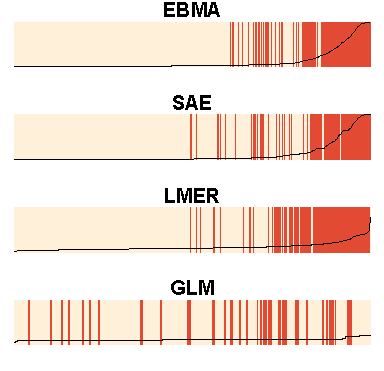
\includegraphics[scale =.4]{Insamplenew.pdf}
\end{center}
\end{wrapfigure}

We compare the models using three other metrics.  The proportional
reduction in error (PRE) is the percentage increase of correctly
predicted observations relative to some pre-defined base model. The
base model in this case is a predicting ``no insurgencies'' for all
observations.  Insurgencies are rare events.  Thus, predicting a
zero for all observations leads to a 89\% correct prediction rate. The Brier
score is the average squared deviation of the prediction from the true
event, thus a lower score corresponds to higher accuracy of forecasts
\citep{Brier:1950}.  Finally, we calculate the percentage of
observations that each model would predict correctly using a 0.5
threshold on the predicted probability scale.

There are two important aspects of Table \ref{InSam1} that are
important to note.  First, the EBMA model does at least as well (and
usually better) than all of the component models on each our model fit
statistics.  The EBMA model has the highest AUC, PRE, and \% correct.
In addition, it is tied for the lowest Brier score with the SAE model.
Second, in this example the EBMA procedure assigns probability weights
to each model according to their in-sample performance.  The highest
model weight (0.57) is assigned to the SAE model, which appears to be
the best (or tied for the best) on all of our fit
statistics. Meanwhile, the lowest weight (0.00) is assigned to the
rudimentary GLM model.


% % latex table generated in R 2.11.1 by xtable 1.5-6 package
% % Sat Mar  5 17:06:38 2011
% \begin{table}[ht]
% \begin{center}
% \caption{model statistics -- in-sample predictions}\label{InSam1}\begin{tabular}{rrrrrrrr}
%   \hline
% & Weight & Constant & Predictor & AUC & PRE & Brier & \% Correct
% \\
%   \hline
% Lmer Politics & 0.48 & 0.19 & 7.88 & 0.97 & 0.41 & 0.04 & 93.28
% \\
%   Glm 1 & 0.00 & 0.61 & 8.32 & 0.61 & 0.00 & 0.10 & 88.65 \\ 
% Lmer Politics 2 & 0.15 & 6.08 & 28.25 & 0.96 & 0.01 & 0.07 &
% 88.79 \\
%   Glm 2 & 0.00 & 0.57 & 8.16 & 0.65 & 0.00 & 0.10 & 88.65 \\ 
%   Lmer 3 & 0.01 & 4.56 & 23.41 & 0.93 & 0.01 & 0.07 & 88.74 \\ 
%   SAE & 0.36 & 0.04 & 7.46 & 0.96 & 0.48 & 0.04 & 94.11 \\ 
%   BMA &  &  &  & 0.98 & 0.48 & 0.04 & 94.11 \\ 
%    \hline
% \end{tabular}
% \end{center}
% \end{table}

Figure \ref{InSam1sep} shows the separation plots for the EBMA model
as well as all the individual components. The plots can be interpreted
as follows. In each plot, the observations are ordered from left to
right by increasing predicted probabilities of insurgency as predicted
by the particular model. The black line corresponds to the predicted
probability produced by the model for each observation. Actual
occurrences of insurgencies are colored red.  Figure \ref{InSam1sep}
shows visually that the GLM model perform very poorly, whereas of the
SAE model is the best component.  More importantly, the overall best
performance is EBMA forecast. The separation plots show that the EBMA
model produces few false positives and even fewer false negatives than
any of the component models.

% latex table generated in R 2.12.0 by xtable 1.5-6 package
% Thu May 12 10:46:44 2011
\begin{table}[h!]
\begin{center}
\caption{\footnotesize Out-of-sample results: Fit statistics for EBMA
    deterministic forecast and all component model forecasts of
    insurgency in 29 countries of the Pacific rim.}\label{OutSam1}
\begin{tabular}{rrrrrrrr}
  \toprule
 & AUC & PRE & Brier & \% Correct \\ 
  \midrule
  SAE &  0.96 & 0.04 & 0.06 & 89.80 \\ 
  LMER & 0.97 & 0.00 & 0.07 & 89.37 \\ 
  GLM & 0.84 & 0.00 & 0.09 & 89.37 \\ 
  EBMA & 0.96 & 0.18 & 0.05 & 91.24 \\ 
   \bottomrule
n=696 \\
\end{tabular}
\end{center}
\end{table}

\begin{wrapfigure}{L}{0.6\textwidth}
\caption{\footnotesize Separation plots for out-of-sample predictions of the ICEWS
  data (n=696).  For each model,
  observations are shown from left to right in order of increasing
  predicted probability (shown as the black line).  Observations where
insurgency actually occurred are shown in red.}
\label{OutSam1sep}
\begin{center}
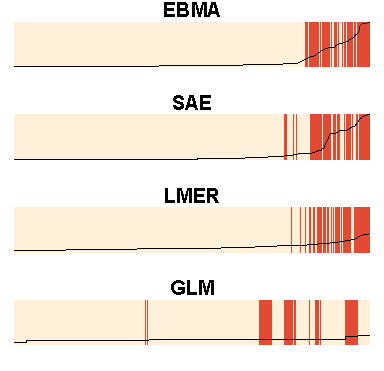
\includegraphics[scale =.4]{OutSampleNew.pdf}
\end{center}
\end{wrapfigure}



The more interesting evaluation of the EBMA method is its
out-of-sample predictive power. Table \ref{OutSam1} shows fit
statistics for the individual components as well as the EBMA forecasts
for observations in the 24 months following the training period.
While the EBMA model has a marginally smaller area under the ROC curve
than the LMER models, it outperforms all component models on any of
the other fit statistics. In particular, the EBMA model has by far the
highest PRE at 0.18.  Since it is possible to predict 89.22\% of these
observations correctly by simply guessing that there is no insurgency,
an 18\% reduction of error relative to the baseline model is quite
substantial.

% % latex table generated in R 2.11.1 by xtable 1.5-6 package
% % Sun Mar  6 14:07:32 2011
% \begin{table}[ht]
% \begin{center}
% \caption{model statistics -- out-of-sample
% predictions}\label{OutSam1}
% \begin{tabular}{rrrrr}
%   \hline
% & AUC & PRE & Brier & \% Correct \\ 
%   \hline
% Lmer Politics & 0.94 & 0.05 & 0.06 & 89.94 \\ 
%   Glm 1& 0.72 & 0.00 & 0.09 & 89.37 \\ 
%   Lmer Politics 2  & 0.97 & 0.00 & 0.07 & 89.37 \\ 
%   Glm 2 & 0.84 & 0.00 & 0.09 & 89.37 \\ 
%   Lmer 3 & 0.97 & 0.00 & 0.07 & 89.37 \\ 
%   SAE & 0.96 & 0.04 & 0.06 & 89.80 \\ 
%   BMA & 0.96 & 0.11 & 0.05 & 90.52 \\ 
%    \hline
% \end{tabular}
% \end{center}
% \end{table}

Figure \ref{OutSam1sep} shows the separation plots for the components
as well as the EBMA forecasts.  The EBMA model performs better than
any of the individual components, with very high predicted
probabilities for the majority of actual events. 

Taking all the evaluation statistics together, as well as the visual
evidence, we can conclude that the EBMA model leads to a substantial
improvement in out-of-sample forecasts relative to its components, even
in datasets with rare events and when individual models are already
performing very well.

\subsection{Application to US presidential election forecasts}
For the past several presidential elections, a number of research
teams have developed forecasting models.  For example, before the most
recent election, a symposium of forecasts was published in \emph{PS:
  Political Science and Politics} with forecasts of presidential and
congressional vote shares developed by \citet{Campbell:2008},
\citet{Norpoth:2008}, \citet{Lewis-Beck:Tien:2008},
\citet{Abramowitz:2008}, \citet{Erikson:Wlezien:2008},
\citet{Holbrook:2008}, \citet{Lockerbie:2008} and
\citet{Cuzan:Bundrick:2008}.  Responses to the forecast and
evaluations were published in a subsequent issue of the
journal.\footnote{In 1999, an entire issue of the
  \textit{International Journal of Forecasting} was dedicated to the
  task of predicting presidential elections \citep{Brown:1999}.}
Predicting presidential elections has also drawn the attention of
economists seeking to understand the relationship between economic
fundamentals and political outcomes.  Two prominent examples include
work by Ray Fair (\citeyear{Fair:2010}) and Douglas Hibbs
(\citeyear{Hibbs:2000}).

\subsubsection{Component Models}

In the rest of this sub-section, we replicate several of these models and
demonstrate the usefulness of the EBMA methodology for improving the
prediction of single important events.  We include six of the most widely cited
presidential forecasting models: 
\begin{itemize}
\item \textbf{Campbell}: Joseph Campbell's ``Trial-Heat and Economy Model''
  \citep{Campbell:2008}.
\item \textbf{Lewis-Beck}: Lewis-Beck and Tien's ``Jobs Model Forecast'' \citep{Lewis-Beck:Tien:2008},
\item \textbf{Erikson}: Erikson and Wlezien's ``Leading Economic Indicators
  and Poll'' forecast,\footnote{We replicated Column 2 in Table 2 from \citet{Erikson:Wlezien:2008}.}
\item \textbf{Fair}: Fair's presidential vote-share model,\footnote{The model here replicates Equation 1 in \citet{Fair:2010}.}
\item \textbf{Hibbs}: Hibbs' ``Bread and Peace Model'' \citep{Hibbs:2000},
\item \textbf{Abramowitz}: and,  the ``Time-for-Change Model'' created by
  \citet{Abramowitz:2008}.  
\end{itemize}

\noindent With the exception of the Hibbs forecast, all of these models are
simple linear regressions.  In all cases, the dependent variable
is the share of the two-party vote received by the candidate from the
incumbent party.  

The data to replicate the models by \citet{Abramowitz:2008,Campbell:2008,Erikson:Wlezien:2008,Lewis-Beck:Tien:2008} were provided to us in personal correspondence with the respective authors. To replicate the \citet{Hibbs:2000} and \citet{Fair:2010} model the data were downloaded from the personal websites of Ray C. Fair \citep{Fair2011} and Douglas Hibbs \citet{Hibbs2011}. 
% this sufficient?

\subsubsection{Results}

Rather than choosing a single training period as in the insurgency
analysis above, here we generate sequential predictions.  For each
year from 1976 to 2008 we use all available prior data to fit the
component model.\footnote{For example, the Fair model uses data for election
  results beginning in 1916 while the Abramowitz model begins with
  data from the 1952 election. }  We then fit the EBMA model using the
components' in-sample performances for election years beginning with
1952 (the year when all models begin generating prediction).  For
example, to generate prediction for the 1988 election we used the
in-sample performance of each component for the 1952-1984 period to
estimate model weights.\footnote{Because of the paucity of data, we
  constrain the predictor, denoted $a_{1k}$ above, to one for all
  models.}

Table \ref{Pres-Year-Res} provides the results of the analysis for the
2008 and 2004 elections.  The table shows the out-of-sample prediction
errors, calculated as $y_{predicted}-y_{observed}$, for each component
model and the EBMA forecast.  Table \ref{Pres-Year-Res} also shows the
weights assigned to each model as well as the in-sample root mean
squared error (RMSE) and mean absolute error (MAE) for the
components and the EBMA forecasts.  A visual representation of the of
the weighted component predictive PDFs and the resulting predictive EBMA PDF is
shown in Figure \ref{PresPlots}.

\begin{table}[ht!]
\caption{\footnotesize Prediction errors, model weights, and in-sample fit
  statistics for component and EBMA forecasts of the 2008 and 2004
  elections.  Models are sequentially fit using all available data
  from prior elections.}
\label{Pres-Year-Res}
\begin{tabular}{l | rrrr||rrrr}	
\toprule
 &\multicolumn{4}{c}{\textit{2008 Election}}  &\multicolumn{4}{c}{\textit{2004 Election}} \\ 
&\shortstack{Pred. \\ Error} &	Weights&	RMSE &MAE & \shortstack{Pred.\\  Error} &Weights&	RMSE&	MAE\\
\midrule
Campbell  &	5.92&	0.34	&1.69&	1.36	&	0.11&	0.29&1.75&	1.45\\
Lewis-Beck&	-1.95&	0.05	&1.64&	1.40	&	0.30	&0.00&	1.70	&1.49\\
Erikson&	-0.11&	0.20&	2.81& 	2.18	&	3.70	&0.21	&2.72&	2.06\\
Fair&	-1.49&	0.00	&2.23&	1.83	&	3.41&	0.10&	2.12& 1.71\\
Hibbs &	-0.93&	0.34	&1.93&	1.33	&	1.50&	0.40	&1.95	&1.32\\
Abramowitz&	-1.88&	0.08	&1.57&	1.30	&	1.92&	0.00	&1.55	&1.25\\
EBMA&	-0.29&	&1.43&	1.08	&	1.59	&	&1.49& 1.09\\
\bottomrule
\end{tabular}
\end{table}

Examining Table \ref{Pres-Year-Res}, it is clear that there is not a
clean relationship between in-sample model performance and model
weights as there was in the insurgency example above.  For instance,
the model weights for the EW model in 2008 is 0.20 even though it has
nearly the highest RMSE and MAE of any component model.  This is
because many of the forecasts are highly correlated.  \footnote{The
  correlation matrix between fitted-values of the model for the
  1952-2008 period is: \\
\begin{tabular}{l | rrrrrr}
  \toprule
 & C& LBT & EW& F & H & A \\ 
  \midrule
Campbell& 1.00 & & & & & \\ 
 Lewis-Beck& 0.93 & 1.00 & & & & \\ 
Erikson & 0.85 & 0.86 & 1.00 & & & \\ 
  Fair & 0.87 & 0.88 & 0.91 & 1.00 & & \\ 
Hibbs& 0.91 & 0.91 & 0.87 & 0.89 & 1.00 & \\ 
  Abramowitz & 0.94 & 0.96 & 0.90 & 0.90 & 0.93 & 1.00 \\ 
   \bottomrule
 \end{tabular}.}  For instance, fitted values for the Abramowitz model are correlated at
0.94 with the Campbell model and at 0.96 with the Lewis-Beck/Tien model.  Thus, conditioned on
knowing the Campbell and Lewis-Beck/Tien forecasts, the Abramowitz forecast provides limited
additional information.  Thus, the bulk of the model weight within
this cluster of predictions is assigned to the Campbell model, which is generally the best predictor.  


\begin{figure}[ht!]
  \caption{\footnotesize Weighted predictive PDF's for component
    models (colored lines) and the full EBMA predictive PDF (thick
    black line).  The ``O'' shows the deterministic EBMA prediction
    and the ``X'' shows the actual observed value for the given year.
    The dashed line is the 95\% credible interval for the EBMA
    predictive PDF.}
\label{PresPlots}
\begin{center}
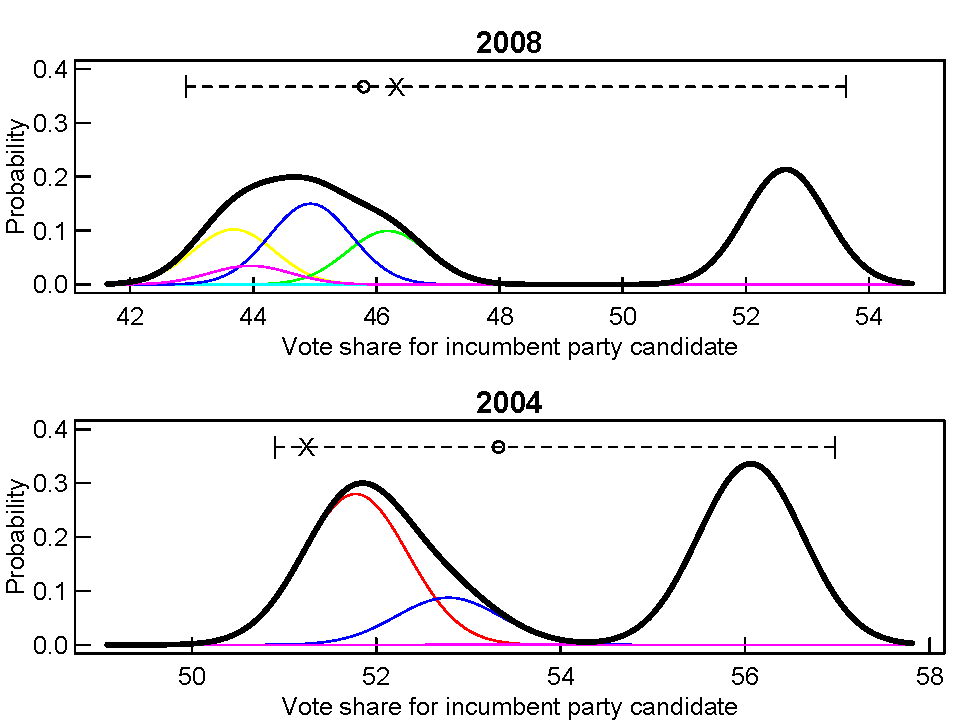
\includegraphics[width=5 in]{PresPlots.PDF}
\end{center}
\end{figure}

With these two examples in mind, we now turn to the relative
out-of-sample performance of the EBMA and component forecasts across
the entire 1976-2008 period.  Table \ref{Pres-Res} shows the both the
RMSE and MAE statistics for each model as well as the percentage of
observations that fall within the 67\% and 95\% predictive credible
intervals for each model.  The last column shows the continuous ranked
probability scores (CRPS) for each probabilistic forecast.  The CRPS
is the integral of the Brier score at all possible threshold values
\citep{Hersbach:2000}.  It is a richer evaluation when considering
predictive distributions rather than point estimates and scores closer
to 0 indicate superior predictive power.  

For our purposes here, the main result apparent in Table
\ref{Pres-Res} is that the EBMA models again outperform all component
models.  The first two columns of Table \ref{Pres-Res} show that this
is true in terms of predicted error (RMSE and MAE).  Moreover, CRPS
statistics show that this is true for the overal predictive PDFs and
not just for the deterministic forecasts.

Just as important, however, the coverage results show much better
calibration of EBMA forecasts relative to the component models.  For
instance, the observed outcome falls within the 95\% predictive
credible interval for the Campbell model only four out of eleven
times.  In general, since the EBMA forecasts is not as sensitive to
particular data issues or events, it is less likely to produce wildly
incorrect predictions.  

An example of the kinds of problems that may arise through reliance on
a single model is seen in the Campbell model.  From 1952 to 2004, this
model was one of the strongest performers.  Indeed, this was the most
accurate forecast of the 2004 election.  However, as a result of the
particularly late timing of the Republican Convention in the 2008
election,\footnote{One of the only two variables in the Campbell model
  comes from polling data measured in early September.  The model also
  relies on 2nd quarter GDP growth, which dramatically fell as the
  election approached due to the financial crisis.  The net result of
  these two factors is that the Campbell model's prediction for 2008
  was one of the largest mis-predictions in the dataset.} it was the
only model to forecast a victory for Republican John McCain.  By
relying on a wider array of data sources and methodologies, the EBMA
method allows us easily ``hedge'' our bets and reduce the likelihood
of such large misses.

\begin{table}[ht!]
  \caption{\footnotesize Fit statistics, observed coverage
    probabilities, and continuous ranked probability scores (CRPS) for
    sequentially generated predictions of presidential elections from 1976-2008.}
\label{Pres-Res}
\begin{tabular}{l|rrrrr}
\hline
	&	RMSE	&	MAE	&	67\% Coverage	&
        95\% Coverage	&	CRPS	\\
\hline
C 	&	2.35	&	1.65	&	0.22	&	0.44	&	1.45	\\
LBT	&	1.81	&	1.52	&	0.11	&	0.33	&	1.29	\\
EW	&	2.41	&	1.88	&	0.22	&	0.33	&	1.68	\\
F	&	2.51	&	2.16	&	0.00	&	0.11	&	1.91	\\
H	&	2.20	&	1.60	&	0.22	&	0.44	&	1.38	\\
A	&	1.84	&	1.62	&	0.11	&	0.22	&	1.39	\\
EBMA	&	1.63	&	1.26	&	0.67	&	0.78
&	0.95	\\
\hline
\end{tabular}
\end{table}


% There should probably be some moving conclusion to this section, but
% I don't know what it should be.  

\subsection{Application to Supreme Court Forecasting Project}

Our final application of EBMA is a re-analysis of forecasts made for
the Supreme Court Forecasting Project \citep{Ruger:2004,
  Martin:2004}.\footnote{Additional details about the project,
  replication files, as well as a complete listing of cases and expert
  forecasts are available at: \url{http://wusct.wustl.edu/index.php}.}
This example highlights the ability of EBMA to handle forecasts not
only generated by statistical models, but also ones provided by
classification trees, subject experts, or other sources.


Throughout 2002-2003, a research team consisting of Andrew
Martin, Kevin Quinn, Theodore Ruger, and Pauline Kim (henceforward
MQRK), generated two sets of forecasts for every pending case.  First,
using data about case characteristics and justices' past voting
patterns, MQRK developed classification trees to generate a binary
forecasts for the expected vote of each justice on each case (voting
to affirm the lower court opinion is coded as a 1).  Second, MQRK
recruited a team of 83 legal experts to make forecasts on particular
cases in their specialty area.  The list included academics, appellate
attorneys, former Supreme Court clerks, and law school deans.  MQRK
attempted to recruit three expert forecasts for each case, although
this was not possible for all cases.

The statistical model makes predictions for all 67 cases included in
the MQRK analysis.  Thus, we include the binary model predictions as
one component forecast. However, the individual legal experts made
predictions on only a handful of cases.  Thus, it is not possible to
calibrate each expert and treat them all as individual ``models.''
Instead, we treat all of the expert opinions as part of a single
forecasting effort.  We coded the expert forecast to be the mean
expert forecast. This implies, that the expert forecast predicts a
vote to affirm if a majority of experts polled for that case predict
an affirming vote.  We fit an EBMA model using all cases with docket
numbers dating from 2001 (n=395).\footnote{For reasons of space, we do
  not present the in-sample results here.  These are available upon
  request.}  We then made EBMA forecasts for the remaining 296 cases
with 2002 docket numbers.

 \subsubsection{Results}

 Table \ref{SC-Res} shows the component weights for the two forecasts
 and the out-of-sample fit statistics for the classification trees,
 subject experts, and EBMA forecasts.  Figure \ref{SCPLOT} provides
 the separation plots.  Once again, the results show that the
 EBMA procedure outperforms all components (even when there are only
 two).  In terms of AUC, Brier scores, and correct predictions, the
 EBMA forecast out-performs both the statistical model and the
 combined subject experts.  In addition, the EBMA forecast offers a
 significantly better PRE.\footnote{The baseline model here is
   prediction that all votes will be to reverse the lower court.  This
   baseline model is correct for roughly 70\% of the votes in the
   out-of-sample period.}

% latex table generated in R 2.12.0 by xtable 1.5-6 package
% Thu May 12 17:11:59 2011
\begin{table}[ht]
\caption{\footnotesize Out-of-sample results: Fit statistics for EBMA deterministic
  forecast and all component model forecasts of Supreme Court votes on
cases in the 2002-2003 session with 2002 docket numbers.  }
\label{SC-Res}
\begin{center}
\begin{tabular}{rrrrrrrr}
  \hline
 & Weight & AUC & PRE & Brier & \% Correct \\ 
  \hline
MQRK model& 0.32  & 0.66 & -0.02 & 0.29 & 70.56 \\ 
Subject experts & 0.68 & 0.62 & 0.15 & 0.23 & 75.23 \\ 
EBMA forecast&  & 0.70 & 0.21 & 0.18 & 77.10 \\ 
   \hline
n=214 \\
\end{tabular}
\end{center}
\end{table}


%\begin{figure}[ht!]
%\caption{\footnotesize Separation plots for out-of-sample predictions
%  of the Suprem Court votes (n=214). For each model, observations are
 % shown from left to right in order of increasing predicted
 % probability (shown as the black line).  Instances where justices voted
  %to affirm the lower court opinion (coded as 1) are colored in red.}
%\label{SCPLOT}
%\begin{center}
%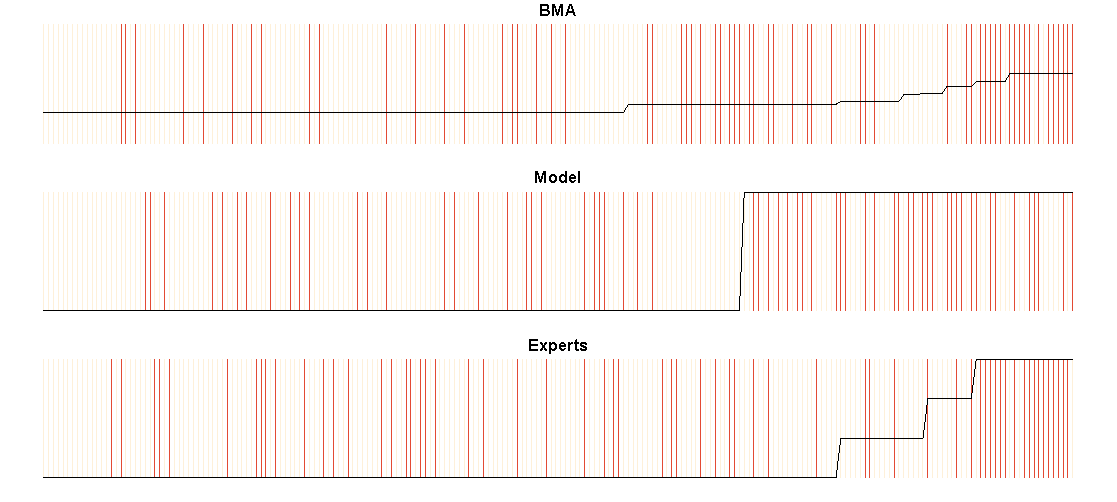
\includegraphics[width=6.5 in]{SCPlot.PDF}
%\end{center}
%\end{figure}

There is a long-standing debate in may circles of the relative
strengths and weaknesses of statistical models and subject experts for
making predictions.  Models that use quantifiable measurements and
widely available (if sometimes crude) data to make comprehensive
predictions can often make egregious errors in particular cases.  In
some cases outcomes may be determined by forces invisible to the
statistical model but obvious to experts familiar with the case.
Subject experts, on the other hand, can often become too focused on
minutia and miss larger (if more subtle) trends in the data that are
easily recognizable by more advanced methodologies.  However, the EBMA
technique offers a theoretically motivated way to combine the
strengths of both methods, while smoothing over their relative
weaknesses, to make more accurate predictions possible.

\section{Proposed research}

In our work so far, we have extended prior research to make EBMA
applicable to binary as well as continuous dependent variables in
political science.  While, as the above examples demonstrate, the
current state of the method already increases the accuracy of
predictions significantly, with support from the NSF we plan to expand
this research in the following ways.

\begin{enumerate}
\item Extend the above into a fully Bayesian framework.  Markov chain
  Monte Carlo estimation of EBMA models promises to more efficiently
  handle a wider variety of predictive distributions and will provide
  additional information regarding our uncertainty  about model
  weights and within-model variances \citep{Vrugt:2008}.
\item The current versions of EBMA estimates model weights exclusively
  based on the point predictions of the component forecasts.  Even for
  continuous data (e.g., the presidential vote forecasts), the current
  procedure assumes that the within-forecast variance ($\sigma^2$) is
  constant across models.  In other words, model weights do no reflect
  the uncertainty associated with each model's predictions.  Applying
  both Bayesian and bootstrap methods, we intend to incorporate the
  entire probability distribution of each of the individual predictive
  models to calibrate model weights.  By using this additional
  information about the component models in the EBMA process, we hope to even further increase
  the performance of the ensemble forecasts.
\item As a result of our research we will develop open-source software
  that will be available for general use.  Specifically, we intend to
  develop an R package that will implement the binary outcome version
  we have already developed and the additional extensions just
  discussed.  Moreover, the package will provide a more flexible
  interface for users interested in ensemble forecasting outside of
  the weather prediction community than is available in the
  `ensembleBMA' package.  The development and free distribution of
  this package will allow researchers in political science and other
  fields to easily employ the EBMA method proposed here.
\item As we specify in our data management plan, all the data used in
  this project will be publicly available for use by other researchers.
\end{enumerate}   

% This should probably end with a re-capitulation of the benefits of
% EBMA and forecasting.  Tell them why they should fund us.

\section{Results from Prior NSF Support}

\section{Results from Prior NSF Support}

\noindent Results from Prior NSF Results during the Previous 5 years

\begin{enumerate}
\item  0827016 (\$749,970; PI's sub \$150,000) AOC: The Dynamics of Secessionist Regions: Eurasian Unrecognized Quasi-States after Kosovo's Independence 10/01/2008--09/30/2011

\item 0631531 (\$400,000) Longitudinal Network Modeling of International Relations Data 11/15/2006--10/31/2009

\item  0433927 (\$650,000; PI's sub \$150,000) The Dynamics of Civil War Outcomes: Bosnia and the North Caucasus 10/01/2004--09/30/2008

\item  0417559 (\$150,000) Network Modeling of International Peace and Trade Data 10/01/2004--09/30/2006 

\item 0631531 () Longitudinal Network Modeling of International Relations Data  
\end{enumerate}

Only one of these grants is still open (\# 1), but these funds have only recently (Spring 2011) been transferred to Duke University. The most relevant grant is \# 5 and below findings and impacts of the project are provided: 
\vspace{.1in}

\textbf{Summary of Findings:} one of our primary findings is that standard hazard regression methods for longitudinal relational data, using variants of proportional hazards models, are unable to properly account for temporal or relational dependence in international relations data. We are developing new methods that are able to account for these dependencies. We have also explored several other approaches to modeling the longitudinal dependencies, one which models the temporal correlations directly, treating them directly as a network and a second which uses the temporal evolution of the latent network as a means of imparting dynamic structure into the estimation of the network parameters. 

A final approach which we are completing now involves modeling a separate time-series regression for each pair of countries, but using a special array-variate hierarchical model to allow for similarity in trade patterns across groups of countries. We have shown that the regularized estimates from the hierarchical model provide better out of sample predictive performance of longitudinal trade data than existing methods. 

\textbf{Broader Impacts:} We have presented the research at a number of conferences and in departmental seminars, in the fields of statistics and biostatistics, as well as political science and geography. We have created the first installment of a series of open-source software packages for the analysis of relational data. These packages are widely used in the social science community undertaking network analysis. In addition we have constructed a database of trade and conflict that can be accessed by this suite of software. 


\noindent In addition, within one year the project completed the following:
\begin{enumerate}

\item  trained a graduate student in the analysis of longitudinal relational data. 

\item constructed and analyzed databases on longitudinal international relations data, including data on conflicts, trade, currency exchange, membership in IGOs and others

\item developed new statistical methodologies for multivariate and longitudinal data. 

\item conducted basic research in the area of multivariate statistical models, including methods related to copula modeling and reduced-rank matrix models. 

\item conducted basic research into the analysis of array data, such as longitudinal trade data, using random-effects versions of multiway array methods such as PARAFAC. Developed an extension of the multivariate and matrix-variate normal distribution appropriate for modeling multiway array data. 

\end{enumerate}

Furthermore, two students learned how to gather and organize data, write technical documents, and perform independent research. Both students completed their Ph.D. in the summer of 2010. One student (John Ahlquist) received two national awards for his dissertation. 
\\

\textbf{Publications Resulting from Award:}

\begin{itemize}

\item Michael D. Ward, Randolph M. Siverson, and Xun Cao.
\newblock Disputes, Democracies, and Dependencies: A Re-examination of the Kantian Peace.
\newblock {\sc American Journal of Political Science}, Volume 51, no. 3 (July), pp. 583-601, 2007.

\item Michael D. Ward and Peter D. Hoff.
\newblock Analyzing Dependencies in Geo-Politics and Geo-Economics.
\newblock In Jacques Fontanel \& Manas Chatterji (editors) {\sc Contributions to Conflict Management, Peace Economics, and Development, Volume 6, War, Peace and Security}, Emerald Publishing, pp. 133-160.

\item  Pavel Krivitsky, Mark Handcock, Adrian Raftery, Peter Hoff, "Representing degree distributions, homophily and clustering in social networks
with latent cluster models", Social Networks, p. , vol. , (2007). Submitted,
\item  Hoff, Peter, "Modeling homophily and stochastic equivalence in symmetric relational data", Advances in Neural Information Processing
Systems 20, p. 667, vol. , (2008). Published,
\item  Hoff, Peter, "Simulation of the matrix Bingham-von Mises-Fisher distribution, with applications to multivariate and relational data", Journal of
Computational and Graphical Statistics, p. , vol. , (2008). Submitted,
\item  Hoff, Peter, "A hierarchical eigenmodel for pooled covariance estimation", Journal of the Royal Statistical Society, Series B, p. , vol. , (2008).
Submitted,

\item Michael D. Ward. 
\newblock Statistical Analysis of International Interdependencies.
\newblock {\sc The International Studies Encyclopaedic Compendium: Scientific Studies of International Processes}, Volume 10, edited by 
Paul F. Diehl and James D. Morrow, pp. 6615-6628, 2010.

\item  Kristin M. Bakke, Xun Cao, John O'Loughlin, \& Michael D. Ward.
\newblock Social Distance in Bosnia and the North Caucasus Region of Russia: Inter-
and intra-ethnic attitudes and identities.
\newblock {\sc Nations and Nationalism}, in press, 2009, Volume 15, Issue 2, pages 227-253.

\item  Peter Hoff, "Hierarchical multilinear models for multiway data", Computational Statistics and Data Analysis, p. , vol. , (2010). 

\item  Peter Hoff and Xiaoyue Niu, "A covariance regression model", Statistica Sinica, p. , vol. , (2010). Submitted,
Books or Other One-time Publications
\item  John S. Ahlquist, "Building and Using Strategic Capacity: Labor Union Confederations and Economic Policy", (2008). Thesis, Published
Bibliography: Doctoral Dissertation, University of Washington, July
\item  Adrian E. Raftery and Michael D. Ward
\newblock {\sc Statistical Methodology: Special Issue on Statistical Methods for the Social Sciences}.
\newblock Elsevier, Volume 8, 2010.

\end{itemize}


\newpage
\setcounter{page}{1}

 \bibliographystyle{apsr}
\bibliography{Flo_Bib,masterEBMA}
%\bibliography{/Users/mw160/Documents/BIBTEXFILES/predictionrefs/predictions2,/Users/mw160/Documents/BIBTEXFILES/2009mdwbib}}



%Contact information for authors:

\end{document}
\bye
